\documentclass[12pt,oneside]{article}

%%%%%%%%%%%%%%%%%%%%%%%%%%%%
%%   Zusaetzliche Pakete  %%
%%%%%%%%%%%%%%%%%%%%%%%%%%%%
\usepackage{acronym}
\usepackage{enumerate}  
\usepackage{a4wide}
\usepackage{fancyhdr}
\usepackage{graphicx}
\usepackage{palatino}
\usepackage{blindtext}
\usepackage{multirow}
\usepackage[ruled,longend]{algorithm2e}
\usepackage{float}
\usepackage{url}
\usepackage{pdfpages}
\usepackage{booktabs}


% für englische Arbeiten "ngerman" durch "english" ersetzen
\usepackage[ngerman]{babel}

\usepackage[T1]{fontenc}
\usepackage[utf8]{inputenc}
\usepackage[utf8]{inputenc}

%Hervorherbung für Links entfernen
%\usepackage[bookmarks]{hyperref}
\usepackage[bookmarks, pdfborder={0 0 0}]{hyperref}

\usepackage[justification=centering]{caption}
\usepackage{csquotes}


%%%%%%%%%%%%%%%%%%%%%%%%%%%
%% Define line spacing   %%
%%%%%%%%%%%%%%%%%%%%%%%%%%%
\usepackage{setspace}
\setlength{\parindent}{0em}
\setlength{\parskip}{0.5em}

\usepackage{enumitem}
\setlist[itemize]{topsep=0pt, partopsep=0pt, itemsep=-1pt, parsep=3pt}
\setlist[enumerate]{topsep=0pt, partopsep=0pt, itemsep=-1pt, parsep=3pt}

\setlist[1]{topsep=2pt, itemsep=3pt, parsep=4pt}
\setlist[2]{topsep=0pt, itemsep=1pt, parsep=2pt}
\setlist[3]{topsep=-1pt, noitemsep}

% Formating the page
\usepackage{microtype}
% Do not allow single lines at the end of a page
\clubpenalty = 10000
% Do not allow single lines at the beginning of a page
\widowpenalty = 10000 \displaywidowpenalty = 10000


%%%%%%%%%%%%%%%%%%%%%%%%%%%
%$ APA Style für Bibtex  %%
%%%%%%%%%%%%%%%%%%%%%%%%%%%
\usepackage[style=apa,natbib=true,backend=biber]{biblatex}

\DefineBibliographyStrings{german}{
  bibliography = {Literaturverzeichnis},
}
\DefineBibliographyStrings{english}{
  bibliography = {References},
}
\bibliography{literatur}

% Note: The following commands need the "url" package
\setcounter{biburlnumpenalty}{100}
\setcounter{biburlucpenalty}{100}
\setcounter{biburllcpenalty}{100}


%%%%%%%%%%%%%%%%%%%%%%%%%%%%%%
%% Definition der Kopfzeile %%
%%%%%%%%%%%%%%%%%%%%%%%%%%%%%%

\pagestyle{fancy}
\fancyhf{}
\cfoot{\thepage}
\setlength{\headheight}{16pt}


%%%%%%%%%%%%%%%%%%%%%%%%%%%%%%%%%%%%%%%%%%%%%%%%%%%%%
%%  Definition des Deckblattes und der Titelseite  %%
%%  Do not edit                                    %%
%%%%%%%%%%%%%%%%%%%%%%%%%%%%%%%%%%%%%%%%%%%%%%%%%%%%%

\newcommand{\UDOTitle}[9]{

  \thispagestyle{empty}
  
\includegraphics[width=3in]{abbildungen/tud_logo_rgb.jpg}
  \vspace*{\stretch{1}}
  \\
  {\parindent0cm
  \rule{\linewidth}{.1ex}}
  \begin{flushright}
    \vspace*{\stretch{1}}
    \sffamily\bfseries\Huge
    #1\\
    \vspace*{\stretch{1}}
    \sffamily\bfseries\large
    #2\\
    \vspace*{\stretch{1}}
  \end{flushright}
  \rule{\linewidth}{.1ex}

  \vspace*{\stretch{1}}
  \begin{center}

    \vspace*{\stretch{1}}
    \large #5\\

    \vspace*{\stretch{1}}
    \large Studiengang: #4 \\[1mm]
    \large Matrikelnummer: #3\\[1mm]
    \large Erstgutachter:  #8 \\[1mm]
    \large Zweitgutachter:  #9 \\[1mm]

    \vspace*{\stretch{1}}
    \large Bearbeitungszeit: #6 -- #7

    \vspace*{\stretch{2}}
    \large Lehrstuhl für Enterprise Computing\\
    \large Fakultät für Informatik\\
  \end{center}
}


%%%%%%%%%%%%%%%%%%%%%%%%%%%%
%%  Beginn des Dokuments  %%
%%%%%%%%%%%%%%%%%%%%%%%%%%%%

\begin{document}
\sloppy

  \UDOTitle
      {Titel der Arbeit}                            % Titel der Arbeit
      {Nachname, Vorname}                           % Vor- und Nachname des Autors
      {1234567}                                     % Matrikelnummer des Autors
      {Bachelor/Master (Angewandte) Informatik}     % Studiengang
      {Seminararbeit/Bachelorarbeit/Masterarbeit}   % Art der Arbeit
      {dd.mm.yyyy}                                  % Tag der Anmeldung
      {dd.mm.yyyy}                                  % Tag der Abgabe
      {Prof. Dr. Christian Janiesch}                % Name des Erstgutachters
      {N.N.}                                        % Name des Zweitgutachters
      
  \clearpage


%%%%%%%%%%%%%%%%%%%%%%%%%%%%
%%  Zusammenfassung   %%
%%%%%%%%%%%%%%%%%%%%%%%%%%%%
\pagenumbering{Roman} 
    \setcounter{page}{1}
    
\markboth{Zusammenfassung}{Zusammenfassung}
\section*{Zusammenfassung}

Die Zusammenfassung dient dem Leser dazu, einen groben Überblick über die Inhalte zu gewinnen (kurze Problemstellung, Herangehensweise, Lösungsansätze und evtl. der Schlüsselerkenntnisse). Der Umfang sollte ca. eine halbe Seite betragen. Auf der nächsten Seite soll eine Übersetzung der Zusammenfassung als Abstract in englischer Sprache erfolgen.

Allgemeiner Hinweis: Die \glqq neue\grqq~Rechtschreibung bietet viele alternative Möglichkeiten der Rechtschreib. Es ist demnach egal, ob Sie z.B. Potenzial mit \glqq z\grqq~oder Potential mit \glqq t\grqq~schreiben. Auch das Komma kann vor einem erweiterten Infinitiv wahlweise gesetzt oder weggelassen werden. Alternative Schreibweisen bedeuten zugleich aber nicht Beliebigkeit. Sie sollten sich also immer konsequent während der gesamten Arbeit für eine Schreibweise entscheiden. Dieses gilt auch für Fachbegriffe.

\clearpage


%%%%%%%%%%%%%%%%%%%%%%%%%%%%
%%  Abstract   %%
%%%%%%%%%%%%%%%%%%%%%%%%%%%%
\markboth{Abstract}{Abstract}
\section*{Abstract (nur bei Bachelor- und Masterthesis)}
Zusammenfassung in englischer Sprache.

\clearpage

\lhead{}

\tableofcontents
\thispagestyle{empty}
\clearpage

\pagenumbering{Roman} 
    \setcounter{page}{3}
    
\addcontentsline{toc}{section}{\listfigurename}
{%
   	\let\oldnumberline\numberline%
   	\renewcommand{\numberline}{\figurename~\oldnumberline}%
   	\listoffigures%
}
\clearpage
    
\addcontentsline{toc}{section}{\listtablename}
{%
   	\let\oldnumberline\numberline%
   	\renewcommand{\numberline}{\tablename~\oldnumberline}%
   	\listoftables%
}
\clearpage

\addcontentsline{toc}{section}{Abkürzungsverzeichnis}
\input{acronym.tex}
\clearpage

% Formelverzeichnis können an dieser Stelle sinnvolle Ergänzungen sein.


%%%%%%%%%%%%%%%%%%%%%%%%%%%%
%%  Einstellungen  %%
%%%%%%%%%%%%%%%%%%%%%%%%%%%%
\cleardoublepage
\pagenumbering{arabic}  
    \setcounter{page}{1}
\lhead{\nouppercase{\leftmark}}


%%%%%%%%%%%%%%%%%%%%%%%%%%%%
%%  Hauptteil  %%
%%%%%%%%%%%%%%%%%%%%%%%%%%%%

%Kapitel mit Seitenumbruch
\include{kapitel/kapitel1}
\section{Grundlagen} \label{grundlagen}

Direkt unterhalb der Hauptkapitel ist jeweils Platz für eine kurze inhaltliche Überleitung.



\subsection{Unterabschnitt}

Die Überschriftenstrukturierung ist hierarchisch. Es empfiehlt sich, die Arbeit so zu strukturieren, dass der Text immer auf der untersten Ebene steht und zugleich auf gleichen Hierarchieebenen inhaltlich auf gleicher Ebene verfasste Texte stehen.
Kapitelüberschriften sind so zu wählen, dass sie sinnvoll den Inhalt des (Unter-) Kapitels als Aussage wiedergeben.
Die Kapitelüberschriften sind in den Formatvorlagen namentlich als Überschrift 1, Überschrift 2, usw. hinterlegt.

Eine Untergliederung bis zur dritten Ebene ist für Bachelor- und Masterarbeiten sinnvoll.
Es empfiehlt sich, eine vierte Ebene (z.B. 2.1.1.1) zu vermeiden, um die Übersichtlichkeit der Gliederung zu wahren.

Ihr Text sollte unter Einbindung von Grafiken und Tabellen in Absätze gegliedert werden.
Dabei ist zu beachten, dass ein Absatz einen thematischen Gedanken erfasst, wobei am Anfang des Absatzes im Regelfall die Kernaussage zu finden ist und von dieser ausgehend durch weitere Erörterungen innerhalb des Absatzes gegliedert wird.




\subsection{Unterabschnitt zwei}

\subsubsection{Unter-Unterabschnitt}

\textbf{So wird dick geschrieben} und \textit{so kursiv}. 
\citet[685]{janiesch2021machine} so wird Autor, Jahr und Seite zitiert.
So wird in Klammern zitiert: \citep[685]{janiesch2021machine}; oder bei mehreren Quellen: (\cites[685]{janiesch2021machine}[289]{herm2021symbolic}).
So wird eine Internetquelle zitiert: \citet{diewi}.

So wird im Dokument referenziert: Kapitel~\ref{einleitung}, Gleichung~\ref{eq:1} zeigt. Es ist empfehlenswert, Referenzierungen und ihr vorstehendes Wort durch eine Tilde $\sim$, welches in \LaTeX~ein geschütztes Leerzeichen darstellt, zu verbinden$\dots$

\begin{equation}
	\sum_{i=1}^N x_i
	\label{eq:1}
\end{equation}

So nutzen Sie Abkürzungen: \ac{AI}, \ac{BPM}, \ac{DSR} Achten Sie darauf, die Abkürzung in der \texttt{acronym.tex} zu definieren und manuell alphabetisch zu sortieren.
Nach der ersten Nutzung werden nur noch die Abkürzungen verwendet: \ac{AI} oder \ac{BPM}.


Das ist eine unsortierte Auflistung:
\begin{itemize}
	\item Element 1
	\item Element 2
\end{itemize}


So fügt man eine Abbildung ein. Durch \texttt{includegraphics} lassen sich \texttt{.jpg}, \texttt{.png}, und \texttt{.pdf} Dateien leicht einbinden.
\begin{figure}[H]
    \centering
    
\includegraphics[width=0.3\textwidth]{abbildungen/tud_logo_rgb.jpg}
    \caption{Logo der TU Dortmund}
    \label{fig:my_label}
\end{figure}

Wichtig ist, Abbildungen immer im Text zu erläutern und im Text auf die Abbildung zu verweisen (siehe Abbildung~\ref{fig:my_label}).
Dies gilt auch für Tabellen. Bei fremden Abbildungen und Tabellen ist zudem die ursprüngliche Quelle anzugeben (z.$\,$B.~in Klammern am Ende der Bezeichnung).


So schreibt man einen Algorithmus.
\BlankLine
\begin{algorithm}[H]
 \KwData{this text}
 \KwResult{how to write algorithm }
 initialization\;
 \While{not at end of this document}{
  read current\;
  \eIf{understand}{
   go to next section\;
   current section becomes this one\;
   }{
   go back to the beginning of current section\;
  }
 }
 \caption{How to write algorithms}
\end{algorithm}
\BlankLine
\BlankLine


\textit{Manchmal} ist ein manueller Seitenumbruch sinnvoll, z.$\,$B.~wenn sonst eine einzelne Zeile vor oder nach einer Tabelle bzw. Abbilung von dieser getrennt würde.

\newpage

So gestaltet man eine Tabelle: 
\begin{table}[H]
	\caption{Beispieltabelle}
	\centering
	\begin{tabular}{lcr}
		\toprule
		\textbf{Animal} 		& \textbf{Description}	& \textbf{Price} (\$)\\
		\midrule
		\midrule
		\multirow{2}{*}{Gnat}	& per gram    			& 13.65\\
								& each        			& 0.01\\
		\midrule
		Gnu      				& stuffed     			& 92.50\\
		Emu       				& stuffed     			& 33.33\\
		Armadillo 				& frozen      			& 8.99\\
		\bottomrule
	\end{tabular}
\end{table}

\subsubsection{Unter-Unterabschnitt zwei}

Ein Abschnitt steht nie allein.
\include{kapitel/kapitel3}


%%%%%%%%%%%%%%%%%%%%%%%%%%%%
%% Literaturverzeichnis wird 
%% automatisch eingefügt
%%%%%%%%%%%%%%%%%%%%%%%%%%%%
\clearpage
\lhead{}
\addcontentsline{toc}{section}{\bibname}
\printbibliography

\newpage
\addcontentsline{toc}{section}{Anhang}
\include{kapitel/anhang.tex}
\clearpage


%%%%%%%%%%%%%%%%%%%%%%%%%%%%
%% Eidesstattliche Erklärung
%% muss angepasst werden 
%% in Erklaerung.tex
%%%%%%%%%%%%%%%%%%%%%%%%%%%%
% bei englischen Arbeiten ist "Eidesstattliche Erklärung" durch "Affidavit" zu ersetzen
%\phantomsection\addcontentsline{toc}{chapter}{Eidesstattliche Erklärung}
\addcontentsline{toc}{section}{Eidesstattliche Erklärung}
\thispagestyle{empty}
% ACHTUNG: Die Affidavit.pdf muss ausgedruckt, handschriftlich ausgefüllt, und eingescannt werden!
% -> Dann die PDF im folgenden Command durch den Scan ersetzen:
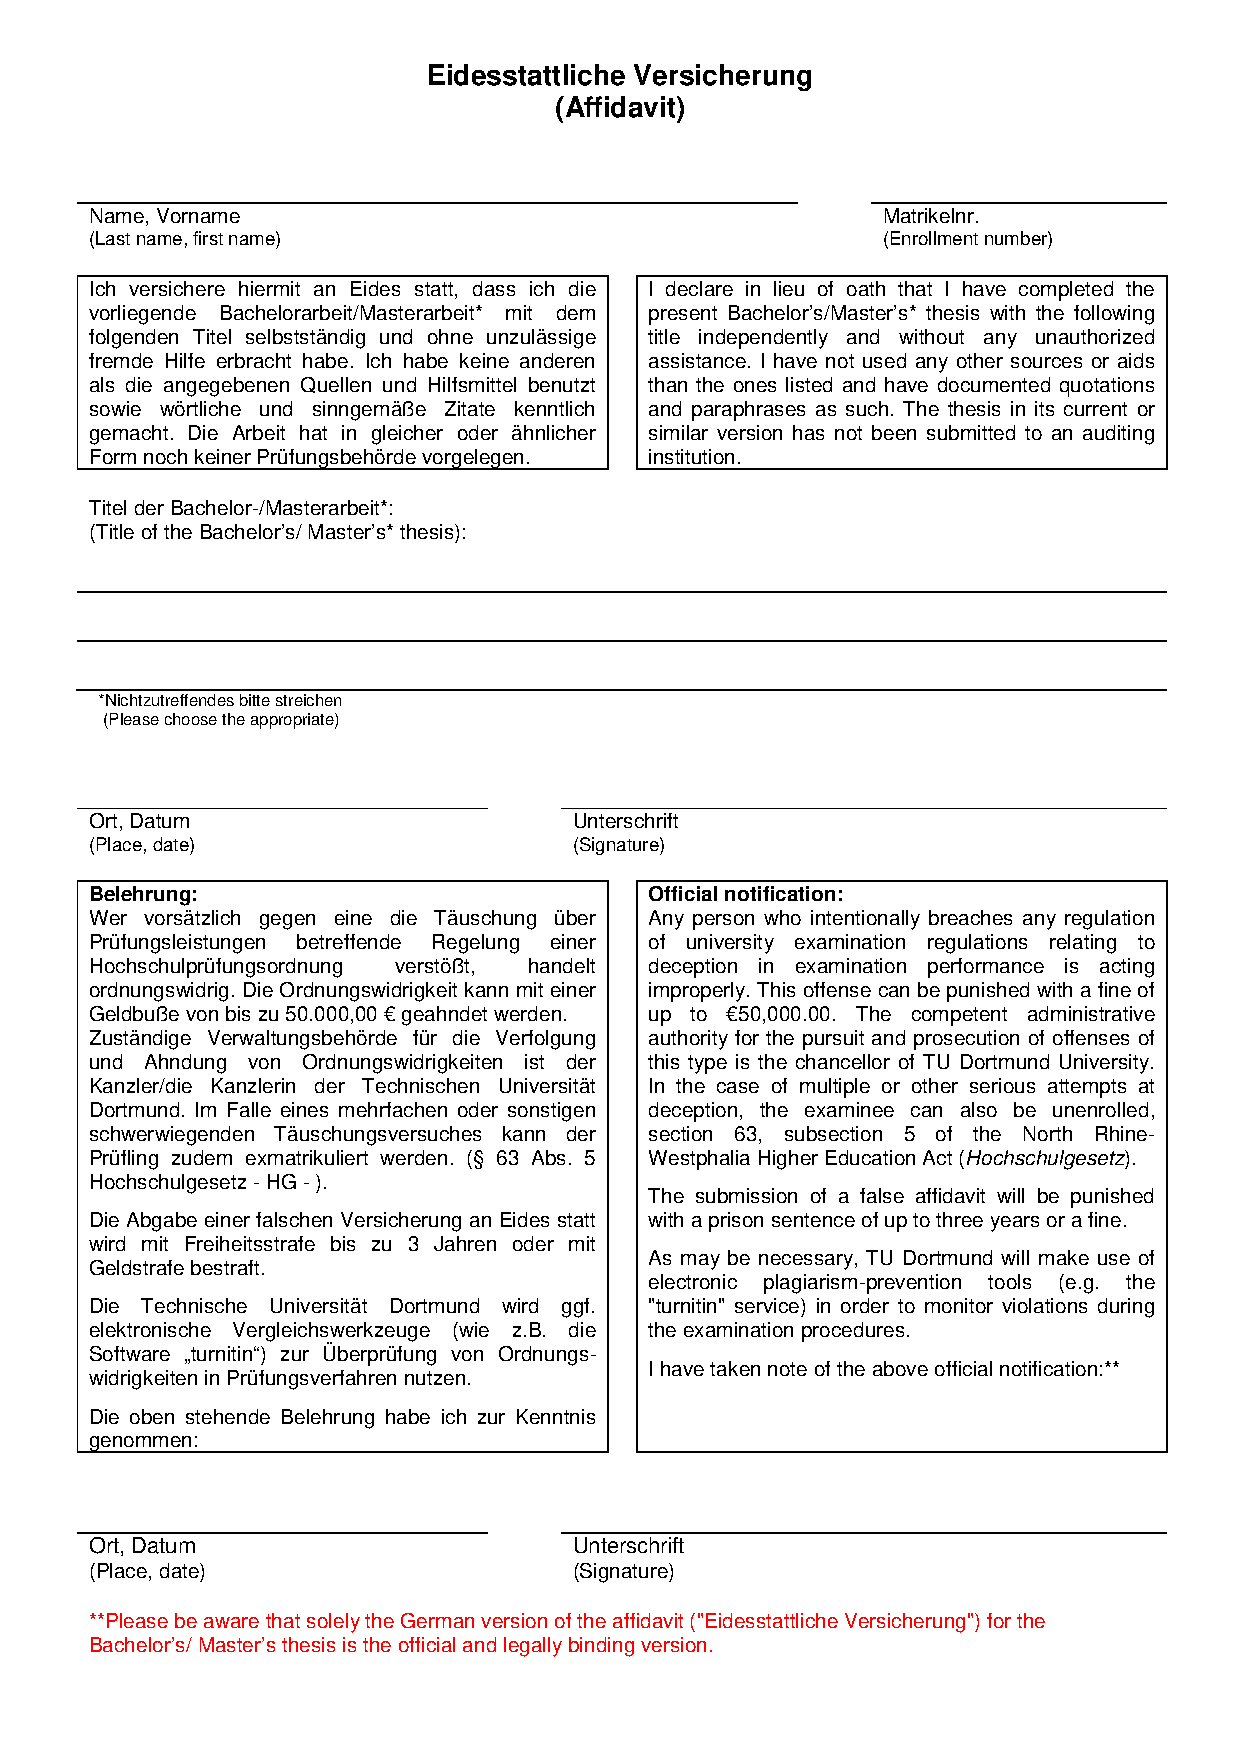
\includepdf{abbildungen/Affidavit.pdf}

\end{document}
